%!TeX root=../tese.tex
%("dica" para o editor de texto: este arquivo é parte de um documento maior)
% para saber mais: https://tex.stackexchange.com/q/78101/183146

%% ------------------------------------------------------------------------- %%
\chapter{ABB estática ótima}
\label{cap:abb-estatica-otima}

Neste capítulo será apresentada a solução para o problema de encontrar uma árvore binária de busca estática com custo mínimo para uma determinada sequência de acessos, ou seja, uma ABB offline estática ótima. O algoritmo foi desenvolvido por \cite{knuth}.

\section{Custo de uma ABB}

O custo de acesso a uma chave em uma ABB estática é o número de nós visitados durante o algoritmo de busca. A \textit{profundidade} de uma chave $j$ em uma ABB $T$ é definida pela distância do nó com chave $j$ à raiz de $T$ e é denotada por $d_T(j)$. Como rotações não são permitidas em ABBs estáticas, a estrutura da árvore não muda, logo o custo de um acesso à chave $j$ numa tal ABB $T$ sempre é 1 mais a profundidade de $j$ em $T$, ou seja, é $1 + d_T(j)$.

O custo de executar uma sequência $X = (x_{1},\ldots,x_{m})$ de $m$ acessos às chaves $1, 2,\ldots,n$ de uma ABB estática $T$ é a somatória dos custos dos acessos executados, ou seja, é
\begin{align*}
c(T) = \sum_{i=1}^{m} (1 + d_T(x_i)).
\end{align*}

Uma delimitação óbvia para este custo é que ele é no mínimo $m$, pois $d_T(j) \geq 0$.

Dada uma sequência $X$ de acessos, uma ABB estática $T$ é considerada ótima para $X$ se $c(T)$ é mínimo, ou seja, se $T$ executa os acessos de $X$ com o menor custo possível.

\section{Natureza do problema}

Definimos o custo para uma sequência de acessos em uma ABB estática com base em cada elemento de $X$. Porém, nota-se que é possível definir o mesmo custo com base no número de ocorrências de cada elemento desta ABB em $X$. Denotaremos por $e(j)$ o número de ocorrências de $j$ na sequência $X$.
Cada acesso ao nó de chave $j$ contribui com $d_T(j) + 1$ ao custo. Como o nó com chave $j$ será acessado $e(j)$ vezes, então o nó de chave $j$ contribui com $(d_T(j) + 1)  \cdot e(j)$ para o custo total, ou seja,
\begin{align*}
c(T) = \sum_{i=1}^{m} (1 + d_T(x_i)) &= \sum_{j=1}^{n} (1 + d_T(j)) \cdot e(j),
\end{align*}
onde a dependência do custo agora é no vetor com o número de ocorrências $e$[1\tdots$n$] de cada chave em $X$.

Essa abordagem também encapsula uma formulação alternativa do problema na qual $e$[1\tdots$n$] representa um vetor de probabilidades de acesso às chaves [1\tdots$n$] na sequência de entrada $X$. Nesse caso a ABB ótima é aquela que possui custo esperado mínimo. Essa é, inclusive, a abordagem utilizada no texto do \cite{knuth}. Nesse artigo também são consideradas probabilidades de buscas mal sucedidas, o que não consideramos no nosso texto. Apesar de limitarmos a análise a buscas bem sucedidas, é possível utilizar a mesma abordagem para resolver problemas que consideram também buscas mal sucedidas.

Dado que a contribuição de cada chave para o custo é uma multiplicação entre a sua profundidade na ABB e seu número de ocorrências na sequência $X$, intuitivamente é esperado que os nós mais próximos da raiz de uma ABB ótima guardem as chaves com os maiores números de ocorrência na sequência, já que a ABB terá que acessar esses nós mais vezes. Analogamente, é esperado que os nós mais distantes da raiz de uma ABB ótima guardem as chaves com os menores números de ocorrência na sequência.

De maneira sucinta, é esperado que o custo de acessos mais caros, ou seja, acessos a nós mais profundos, sejam pagos menos vezes e é esperado que os custos de nós mais baratos, ou seja, acessos a nós mais superficiais, sejam pagos mais vezes.

\section{Algoritmo guloso}

É possível desenvolver um algoritmo guloso para a construção de uma ABB estática com base na intuição de priorizar que chaves com maior número de ocorrência estejam mais próximas da raiz. O Programa~\ref{prog:abb-gulosa} organiza as chaves de maneira decrescente no número de ocorrências e adiciona iterativamente à árvore a chave de maior número de ocorrências que ainda não foi adicionada. Para isso, ele utiliza uma fila de prioridades de máximo que armazena pares ($j$, $e[j]$), considerando o segundo valor do par como prioridade.

\begin{programruledcaption}{Algoritmo guloso ABB.\label{prog:abb-gulosa}}
  \noindent\textbf{Entrada}: Número $n$ de chaves e vetor $e$[1\tdots$n$] de ocorrências por chave. \\
  \textbf{Saída}: ABB com as chaves 1 a $n$ com respeito ao vetor $e$.
  \vspace{-0.5\baselineskip}
  \begin{lstlisting}[
      language={[brazilian]pseudocode},
      style=pseudocode,
      style=wider,
      functions={},
      specialidentifiers={},
      escapeinside={(*@}{@*)},
  ]
  (*@\bfseries\scshape{Função}@*) guloso_ABB(n,e)
    Q := fila_de_prioridade(e, n) (*@ \hfill @*) // Cria uma fila de prioridade para o vetor e[1\tdots$n$]
    abb := abb() (*@ \hfill @*) // Cria uma ABB vazia
    enquanto Q != (*@$\varnothing$@*) 
        (a,b) := Q.remove_max()
        abb.insere(a) (*@ \hfill @*) // Adiciona chave com maior número de ocorrências em Q
  devolva abb
  \end{lstlisting}
  \vspace{-0.5\baselineskip}
\end{programruledcaption}

Apesar da abordagem acima ser bastante promissora, priorizar unicamente o número de ocorrências não garante adquirir uma ABB ótima. Isso acontece porque a posição de cada nó na árvore influencia a profundidade de todos os nós descendentes dele, principalmente levando em conta a propriedade de árvores binárias que exige que todos os nós da subárvore esquerda sejam menores que o nó e todos os nós da subárvore direita sejam maiores. Assim, em algumas situações, é mais vantajoso ter como pai um nó com menor número de ocorrências e ter nós com maior número de ocorrências mais profundos. Isto se torna ainda mais evidente quando pensamos em entradas com número de ocorrências por nó muito parecidos. Nestes casos, a estrutura de uma árvore binária mais balanceada tende a ser melhor. Veja o exemplo da Figura~\ref{fig:caso-guloso-subotimo}.


\begin{figure}[h]
  \centering
  \begin{minipage}[c]{0.35\textwidth}
    \centering
    \begin{tabular}{|c|c|}
    \hline
    \multicolumn{2}{|c|}{\textbf{Número de ocorrências}} \\
    \hline
    \textbf{$a$} & 5 \\
    $b$ & 25 \\
    $c$ & 20 \\
    $d$ & 15 \\
    \hline
    \end{tabular}
    \end{minipage}
  \begin{minipage}[c]{0.3\textwidth}
  \centering
  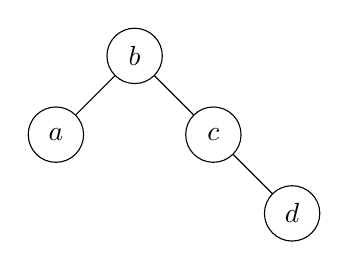
\begin{tikzpicture}
    [node/.style={circle,draw,minimum size=2em}]
    \node[node] (A) at (-1,-1) {$a$};
    \node[node] (B) at (0,0) {$b$};
    \node[node] (C) at (1,-1) {$c$};
    \node[node] (D) at (2,-2) {$d$};
    
    \draw (A) -- (B);
    \draw (B) -- (C);
    \draw (C) -- (D);
  \end{tikzpicture}
  \end{minipage}
  \begin{minipage}[c]{0.3\textwidth}
  \centering
  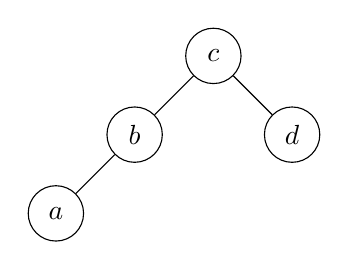
\begin{tikzpicture}
    [node/.style={circle,draw,minimum size=2em}]
    \node[node] (A) at (-2,-2) {$a$};
    \node[node] (B) at (-1,-1) {$b$};
    \node[node] (C) at (0,0) {$c$};
    \node[node] (D) at (1,-1) {$d$};
    
    \draw (A) -- (B);
    \draw (B) -- (C);
    \draw (C) -- (D);
  \end{tikzpicture}
  \end{minipage}
  \caption{Tabela com o número de ocorrências por chave em uma sequência de entrada. À esquerda, a árvore gerada pelo algoritmo guloso, com custo total 120, e à direita, a árvore ótima, com custo total 115.}
\label{fig:caso-guloso-subotimo}
\end{figure}

\section{Algoritmo de Knuth}

A análise da seção anterior nos leva a perceber que precisamos de uma conduta que considere tanto o número de ocorrências de cada nó quanto a estrutura da árvore em si. Um algoritmo para encontrar uma ABB estática ótima foi desenvolvido por \cite{knuth}.

Primeiramente é preciso entender como a estrutura de uma árvore ótima está disposta.

Lembremos que a profundidade de uma chave $i$ em uma ABB $T$, é a distância, $d_T(i)$, entre o nó com chave $i$ e a raiz de $T$. Assim sabemos que se a chave $i$ está na subárvore $T'$ de $T$, então a distância do nó com chave $i$ à raiz de $T$ é a distância do nó com chave $i$ à raiz de $T'$ adicionada à distância da raiz de $T'$ à raiz de $T$. Suponha que a chave $j$ seja raiz de $T'$. Então, $d_T(i) = d_{T'}(i) + d_{T}(j)$.

Seja $T$ uma ABB estática ótima com $n$ chaves para uma sequência de acessos $X$. Seja $k$ a chave da raiz de $T$ e $T_e$ e $T_d$ as subárvores esquerdas e direitas da raiz. Como $k$ é a chave da raiz, $T_e$ possui as chaves \{$1,\ldots,k-1$\} e $T_d$ possui as chaves \{$k+1,\ldots,n$\}. 

Como $T_e$ é a subárvore esquerda da raiz de $T$, a profundidade em $T$ da raiz de $T_e$ é~1. Logo, para qualquer chave $i \in T_e$, $d_T(i) = d_{T_{e}}(i) + 1$. O caso de $T_d$ é análogo. Ademais, $d_T(k) = 0$, pois $k$ é a chave da raiz.

Assim,
\begin{align*}
  c(T) &= \sum_{j=1}^{n}(d_T(j) + 1)\cdot e(j) \\
  &= \sum_{j=1}^{k-1}(d_T(j) + 1) \cdot e(j) + \sum_{j=k+1}^{n}(d_T(j) + 1)\cdot e(j) + (d_T(k) + 1)\cdot e(k) \\
  &= \sum_{j=1}^{k-1}d_T(j) \cdot e(j) + \sum_{j=k+1}^{n}d_T(j)\cdot e(j) + \sum_{j=1}^{n} e(j) \\
  &= \sum_{j=1}^{k-1}(d_{T_e}(j) + 1)\cdot e(j) + \sum_{j=k+1}^{n}(d_{T_d}(j) + 1)\cdot e(j) + \sum_{j=1}^{n} e(j) \\
  &= c(T_e) + c(T_d) + \sum_{j=1}^{n}e(j),
\end{align*}
onde $c(T_e)$ considera apenas os acessos de $X$ em $\{1,\ldots,k-1\}$, ou seja, considera $e[1 \tdots k-1]$, e $c(T_d)$ considera apenas os acessos de $X$ em $\{k+1,\ldots,n\}$, ou seja, considera $e[k+1 \tdots n]$.

De acordo com a fórmula acima, é evidente que o custo total de uma ABB $T$ depende do custo de suas duas subárvores $T_e$ e $T_d$. Logo para uma árvore $T$ ter custo mínimo então tanto a sua subárvore esquerda quanto a sua subárvore direita devem ter custo mínimo, ou seja, $T_e$ e $T_d$ devem ser ABBs ótimas para as buscas nas chaves que armazenam.

Expressaremos por $c[i,j]$ o custo mínimo de uma ABB que guarda as chaves de $i$ a $j$ em relação ao vetor de ocorrências $e[i \tdots j]$ e por $s[i,j]$ a soma do número de ocorrências de todas as chaves entre $i$ e $j$ em $X$, ou seja, $s[i,j] = \sum_{h=i}^{j} e(h)$.

Chegamos na recorrência abaixo que resolve o problema:
\[
c[i, j] = 
\begin{cases}
    0 & \text{se } i > j. \\
    \min_{i \leq k \leq j} \{ c[i, k - 1] + c[k + 1, j]\} + s[i, j] & \text{se } i \leq j.
\end{cases}
\]

O Programa~\ref{prog:abb-otima} produz uma ABB estática com custo mínimo dado o vetor de ocorrências por chave.

\begin{programruledcaption}{Construção recursiva da ABB ótima.\label{prog:abb-construcao}}
  \noindent\textbf{Entrada}: Dois inteiros $i$ e $j$ e a matriz de inteiros $r$[1\tdots$n$,1\tdots$n$] construída pelo Programa~\ref{prog:abb-otima}. \\
  \textbf{Saída}: ABB estática ótima com as chaves [$i$\tdots$j$].
  \vspace{-0.5\baselineskip}
  \begin{lstlisting}[
      language={[brazilian]pseudocode},
      style=pseudocode,
      style=wider,
      functions={},
      specialidentifiers={},
      escapeinside={(*@}{@*)},
  ]
  (*@\bfseries\scshape{Função}@*) construção_recursiva(i, j, r)
    se i > j
        (*@\textbf{então}@*) devolva NULL
    k := r[i, j]
    nó := novoNó(k)
    nó.esq := construção_recursiva(i, k - 1, r)
    nó.dir := construção_recursiva(k + 1, j, r)
  devolva nó
  \end{lstlisting}
  \vspace{-0.5\baselineskip}
\end{programruledcaption}

\begin{programruledcaption}{Algoritmo de Knuth.\label{prog:abb-otima}}
  \noindent\textbf{Entrada}: Número $n$ de chaves e vetor $e$[1\tdots$n$] de ocorrências por chave. \\
  \textbf{Saída}: ABB estática ótima com chaves 1 a $n$ e seu custo com respeito ao vetor $e$.
  \vspace{-0.5\baselineskip}
  \begin{lstlisting}[
      language={[brazilian]pseudocode},
      style=pseudocode,
      style=wider,
      functions={},
      specialidentifiers={},
      escapeinside={(*@}{@*)},
  ]
  (*@\bfseries\scshape{Função}@*) Knuth(n,e)
    s[0] := 0
    para i de 1 até n (*@\textbf{faça}@*)
        s[i] := s[i - 1] + e[i]
    para i de 1 até n + 1 (*@\textbf{faça}@*)
        c[i, i - 1] := 0
    para (*@{$\ell$}@*) de 1 até n (*@\textbf{faça}@*)
        para i de 1 até n - (*@{$\ell$}@*) + 1 (*@\textbf{faça}@*)
            j := i + (*@{$\ell$}@*) - 1
            c[i, j] := c[i + 1, j]
            r[i, j] := i
            para k de i + 1 até j (*@\textbf{faça}@*)
                se c[i, k - 1] + c[k + 1, j] < c[i, j]
                    (*@\textbf{então}@*) c[i, j] := c[i, k - 1] + c[k + 1, j]
                        (*@\hspace{1em}@*)r[i, j] := k
            c[i, j] := c[i, j] + s[j] - s[i - 1]
    abb := construção_recursiva(1, n, r)
  devolva abb, c[1,n]
  \end{lstlisting}
  \vspace{-0.5\baselineskip}
\end{programruledcaption}

Como o Programa~\ref{prog:abb-construcao} é utilizado pelo Programa~\ref{prog:abb-otima}, então é necessário analisar a construção antes do algoritmo de Knuth.

O Programa~\ref{prog:abb-construcao} recursivamente constrói a ABB. Isso é feito por meio de uma estratégia recursiva de baixo para cima. Assim, a função será executada uma vez para cada nó da ABB e mais uma vez para cada intervalo vazio. Como há exatamente $n$ nós no intervalo de $[1 \tdots n]$, e há $n+1$ intervalos vazios (que correspondem a chamadas da função com $i<j$) produzidos recursivamente, então o custo total do algoritmo é \( \mathcal{O}(n) \).

O Programa~\ref{prog:abb-otima}, por sua vez, adota uma estratégia de programação dinâmica. Esse tipo de estratégia se utiliza de espaço adicional de memória. Neste caso uma matriz, para armazenar computações já executadas. Dessa maneira, evita-se cálculos repetidos e maximiza-se a eficiência do programa.

Para preencher os elementos necessários da matriz para alcançar o custo final, o código itera por metade da matriz. Então serão necessárias \( \mathcal{O}(n^2) \) iterações. A iteração que preenche a posição $[i,j]$ das matrizes $c$ e $r$ representa o cálculo do custo mínimo para uma ABB que contenha todos os elementos do intervalo $[i \tdots j]$. Esse cálculo verifica todas as possíveis raízes, o que é feito nas linhas 12-15 do Programa~\ref{prog:abb-otima}, então tem custo \( \mathcal{O}(n) \). Como há \( \mathcal{O}(n^2) \) iterações de custo \( \mathcal{O}(n) \), o custo total do algoritmo é \( \mathcal{O}(n^3) \). 



